\section{可测映射与可测函数}
\label{sec:measure-measurable-maps}

有了测度，我们还要处理定义在可测空间上的映射：随机实验的结果被读成一个数，平面上的点被投影到坐标轴，一列函数取逐点极限。每当对映射的输出提出“是否落在某集合中”的问题，就需要输入端能够测量相应的点集。本节用原像刻画这一要求，先给出一般可测映射的判据与复合规则，再专门研究实值可测函数，证明常见运算与可数极限保持可测性。用简单函数逼近一般可测函数的构造，留到第~\ref{chap:integration}章定义积分时展开。

\subsection{原像判据与可测复合}
\label{sec:measure-preimage-criterion}

\paragraph{可测映射的定义}
对映射$f:X\to Y$与$B\subseteq Y$，原像$f^{-1}(B)=\{x\in X:f(x)\in B\}$是“输出落在$B$中”的那些输入。原像记号对任意映射都有意义，并不要求$f$可逆（可参考\BookChapterRef{chap:sets-relations-maps}{卷一“集合、关系与映射”章}）。若输出端能提出的每个集合问题，在输入端都对应一个可测集合，就说$f$是可测的。

\begin{definition}[可测映射]
\label{def:measure-measurable-map}
设$(X,\mathcal A)$、$(Y,\mathcal B)$是可测空间。若对每个$B\in\mathcal B$都有$f^{-1}(B)\in\mathcal A$，称映射$f:X\to Y$为$\mathcal A/\mathcal B$-\term{可测映射}（measurable map），简称可测。
\end{definition}

可测性同时取决于两端的$\sigma$代数。在$X=\{1,2,3,4\}$上取由$\varnothing$、$\{1,2\}$、$\{3,4\}$、$X$组成的$\sigma$代数$\mathcal A$，在$Y=\{a,b\}$上取$\mathcal P(Y)$。令$f(1)=f(2)=a$、$f(3)=f(4)=b$，则$f^{-1}(\{a\})=\{1,2\}$、$f^{-1}(\{b\})=\{3,4\}$都可测，$f$可测。令$g(1)=a$、$g(2)=g(3)=g(4)=b$，则$g^{-1}(\{a\})=\{1\}\notin\mathcal A$，$g$不可测：输入端只知道点属于哪一组，无法回答“输出是否为$a$”。若把$Y$上的$\sigma$代数换成$\{\varnothing,Y\}$，$g$又变成可测的，因为输出端不再提出任何非平凡问题。

\paragraph{生成族判据}
直接检查$\mathcal B$中的每个集合往往不可行，例如$\mathcal B(\mathbb R)$中的集合无法逐一列出。原像与集合运算可交换，这使我们只需检查生成族。

\begin{lemma}[生成族判据]
\label{lem:measure-generator-criterion}
设$\mathcal B=\sigma(\mathcal C)$。若对每个$C\in\mathcal C$都有$f^{-1}(C)\in\mathcal A$，则$f$是$\mathcal A/\mathcal B$可测的。
\end{lemma}

\begin{proof}
令$\mathcal E=\{B\subseteq Y:f^{-1}(B)\in\mathcal A\}$。由$f^{-1}(Y)=X$、$f^{-1}(Y\setminus B)=X\setminus f^{-1}(B)$与$f^{-1}(\bigcup_nB_n)=\bigcup_nf^{-1}(B_n)$，$\mathcal E$是$Y$上的$\sigma$代数。它含$\mathcal C$，所以含$\sigma(\mathcal C)=\mathcal B$。
\end{proof}

图~\ref{fig:measure-preimage-criterion}示意了这一判据：只要生成族中每个集合的原像都落在$\mathcal A$中，由补集与可数并生成的其余集合，其原像也由相应运算得到，自动落在$\mathcal A$中。

\begin{figure}[!htbp]
  \centering
  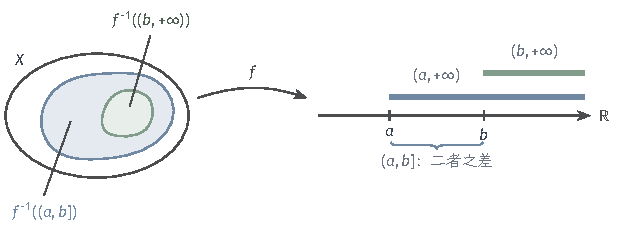
\includegraphics[width=105.1mm]{figures/02-abstract-mathematics/01-metric-and-measure/tikz/c2-preimage-criterion/figure.pdf}
  \caption{原像判据。右侧是输出空间$\mathbb R$中的生成集合$(a,+\infty)$与$(b,+\infty)$，左侧是它们在输入空间$X$中的原像。原像保持集合运算：$(a,b]=(a,+\infty)\setminus(b,+\infty)$的原像等于两个原像之差，所以只要生成集合的原像可测，由它们运算得到的集合，原像也可测。}
  \label{fig:measure-preimage-criterion}
\end{figure}

\paragraph{复合与连续映射}
若$f:(X,\mathcal A)\to(Y,\mathcal B)$与$g:(Y,\mathcal B)\to(Z,\mathcal C)$都可测，则对$C\in\mathcal C$，
\[
 (g\circ f)^{-1}(C)=f^{-1}\bigl(g^{-1}(C)\bigr),
\]
其中$g^{-1}(C)\in\mathcal B$，再由$f$可测得$f^{-1}(g^{-1}(C))\in\mathcal A$，所以复合$g\circ f$可测。这里要求中间空间$Y$上两次使用的是同一个$\sigma$代数$\mathcal B$。

设$(X,d_X)$、$(Y,d_Y)$是度量空间，$f$连续。由第~\ref{sec:metric-continuous-maps}节，开集的原像是开集，因而属于$\mathcal B(X)$；开集生成$\mathcal B(Y)$，由引理~\ref{lem:measure-generator-criterion}，$f$是$\mathcal B(X)/\mathcal B(Y)$可测的。这个结论依赖两端都取Borel结构。若把两端都换成Lebesgue可测集$\mathcal L$，连续函数$f:\mathbb R\to\mathbb R$未必$\mathcal L/\mathcal L$可测：可以构造连续严格单调的函数$f$与Lebesgue零测集的子集$S$（由完备性，$S\in\mathcal L$），使$f^{-1}(S)$不是Lebesgue可测集。这里不展开构造，只记住：可测性必须写清两端的集合族，不能把目标端的Borel结构随意换成某个测度的完备化。

\subsection{可测函数的运算}
\label{sec:measure-function-operations}

\paragraph{阈值判据}
最常用的可测映射是取实数值的函数。目标端取$\mathcal B(\mathbb R)$，由定理~\ref{thm:measure-borel-generators}，半直线$(a,+\infty)$生成它，判据化为检查阈值集合。

\begin{definition}[可测函数]
\label{def:measure-measurable-function}
设$(X,\mathcal A)$是可测空间。若$f:X\to\mathbb R$是$\mathcal A/\mathcal B(\mathbb R)$可测的，称$f$为\term{可测函数}（measurable function）。对取值于扩展实数$[-\infty,+\infty]$的函数，若对每个$a\in\mathbb R$都有$\{f>a\}=\{x:f(x)>a\}\in\mathcal A$，也称它可测。当$(X,\mathcal A)=(\mathbb R^d,\mathcal B(\mathbb R^d))$时，称为\term{Borel可测函数}（Borel measurable function）。
\end{definition}

\begin{lemma}[阈值判据]
\label{lem:measure-threshold}
$f:X\to\mathbb R$可测，当且仅当对每个有理数$a$，$\{f>a\}\in\mathcal A$。
\end{lemma}

\begin{proof}
必要性：$\{f>a\}=f^{-1}((a,+\infty))$。充分性：由定理~\ref{thm:measure-borel-generators}，有理端点半直线$(a,+\infty)$生成$\mathcal B(\mathbb R)$，再用引理~\ref{lem:measure-generator-criterion}。
\end{proof}

用补集与可数运算还可得到其他阈值集合，例如$\{f\ge a\}=\bigcap_n\{f>a-1/n\}$、$\{f\le a\}=X\setminus\{f>a\}$，它们也都可测。

\paragraph{示性函数与简单函数}
集合可测性与函数可测性通过指示函数相连。对$A\subseteq X$，$\{\mathbf 1_A>a\}$在$a<0$时为$X$，在$0\le a<1$时为$A$，在$a\ge1$时为$\varnothing$，所以$\mathbf 1_A$可测当且仅当$A\in\mathcal A$。例如$\mathbf 1_{\mathbb Q}$在$(\mathbb R,\mathcal B(\mathbb R))$上可测，因为$\mathbb Q$是Borel集；第~\ref{sec:measure-jordan}小节中它对应的集合连Jordan可测都不是，测度论却可以直接处理它。

\begin{definition}[简单函数]
\label{def:measure-simple-function}
只取有限多个实数值的可测函数称为\term{简单函数}（simple function）。
\end{definition}

设简单函数$\varphi$的不同取值为$c_1,\dots,c_m$，令$A_i=\varphi^{-1}(\{c_i\})$，它们是可测集合，两两不交，并为$X$，于是
\[
 \varphi=\sum_{i=1}^mc_i\mathbf 1_{A_i}.
\]
反过来，任意可测集合$B_j$的有限线性组合$\sum_jb_j\mathbf 1_{B_j}$只取有限多个值，每个取值集合都是若干$B_j$及其补集的交之并，因此是简单函数。同一个简单函数可以有多种写法，例如$\mathbf 1_{[0,2]}=\mathbf 1_{[0,1]}+\mathbf 1_{(1,2]}$；按不同取值写出的上式是标准写法。第~\ref{chap:integration}章将先对简单函数定义积分，再用简单函数逼近一般可测函数。

\paragraph{代数运算}
可测函数经过加、乘、取绝对值等运算后仍然可测。困难在于和的阈值集合$\{f+g>a\}$不能直接写成$f$与$g$各自阈值集合的有限组合，需要用有理数作可数分拆。

\begin{theorem}[可测函数的运算]
\label{thm:measure-function-operations}
设$f,g:X\to\mathbb R$可测，$c\in\mathbb R$，$\varphi:\mathbb R\to\mathbb R$连续。则$cf$、$f+g$、$\varphi\circ f$、$fg$、$|f|$、$\max\{f,g\}$、$\min\{f,g\}$都可测；若$g$处处不为零，$f/g$也可测。
\end{theorem}

\begin{proof}
$\varphi\circ f$是可测映射与Borel可测的连续映射之复合，由上一小节可测。取$\varphi(t)=ct$与$\varphi(t)=|t|$，得$cf$与$|f|$可测；取$\varphi(t)=t^2$，得$f^2$可测。

对和，若$f(x)+g(x)>a$，则$f(x)>a-g(x)$，在两者之间取有理数$q$，有$f(x)>q$且$g(x)>a-q$；反之这两式蕴含$f(x)+g(x)>a$。所以
\[
 \{f+g>a\}=\bigcup_{q\in\mathbb Q}\bigl(\{f>q\}\cap\{g>a-q\}\bigr),
\]
是可数个可测集合之并。于是$f-g=f+(-1)g$也可测。积由恒等式$fg=\tfrac14\bigl((f+g)^2-(f-g)^2\bigr)$得到，最大值与最小值由$\max\{f,g\}=\tfrac12(f+g+|f-g|)$与$\min\{f,g\}=\tfrac12(f+g-|f-g|)$得到。若$g$处处非零，$g$是到$\mathbb R\setminus\{0\}$的可测映射，$t\mapsto1/t$在$\mathbb R\setminus\{0\}$上连续，所以$1/g$可测，$f/g=f\cdot(1/g)$可测。
\end{proof}

允许取扩展实数值时，运算本身可能无定义。$f+g$在$f(x)=+\infty$、$g(x)=-\infty$的点没有意义，必须先说明这样的点不出现，或者在那里另作约定；乘积还要约定$0\cdot(\pm\infty)$。只有在这些点上的值被确定以后，才能谈论运算结果是否可测，不能把形式上的式子当作已经定义好的函数。

\subsection{函数列的可测性}
\label{sec:measure-function-sequences}

\paragraph{可数极限}
分析中的许多函数是作为函数列的极限得到的，例如级数的和与逐次逼近的结果。下面的定理说明，可数个可测函数取上确界、下确界和极限后仍然可测。

\begin{theorem}[可数极限的可测性]
\label{thm:measure-limits}
设$f_1,f_2,\dots:X\to[-\infty,+\infty]$可测。则$\sup_nf_n$、$\inf_nf_n$、$\limsup_nf_n$、$\liminf_nf_n$可测。若对每个$x$，极限$\lim_nf_n(x)$在$[-\infty,+\infty]$中存在，则极限函数可测。
\end{theorem}

\begin{proof}
$\sup_nf_n(x)>a$当且仅当某个$f_n(x)>a$，所以$\{\sup_nf_n>a\}=\bigcup_n\{f_n>a\}$可测。对下确界，$\{\inf_nf_n\ge a\}=\bigcap_n\{f_n\ge a\}$可测，从而$\{\inf_nf_n>a\}=\bigcup_k\{\inf_nf_n\ge a+1/k\}$可测。上极限与下极限是可数次上、下确界的组合：
\[
 \limsup_{n\to\infty}f_n=\inf_{n\ge1}\sup_{k\ge n}f_k,\qquad \liminf_{n\to\infty}f_n=\sup_{n\ge1}\inf_{k\ge n}f_k,
\]
由前两步可测。极限存在时它等于上极限，因而可测。
\end{proof}

这个定理只保证极限对象是可测函数，可以对它提出测度与积分的问题；它并没有说极限函数的积分等于积分的极限。这种交换需要另外的条件，是第~\ref{chap:integration}章收敛定理的内容。

\paragraph{零测修改}
函数在零测集上的取值通常无关紧要，但修改后的函数是否仍然可测，取决于测度空间是否完备。设$f$可测，$g$与$f$仅在某个零测集$N$内的点上可能不同。若空间完备，则
\[
 \{g>a\}=\bigl(\{f>a\}\setminus N\bigr)\cup\bigl(\{g>a\}\cap N\bigr),
\]
第一项可测，第二项是零测集的子集，由完备性可测，所以$g$可测。若空间不完备，结论可能失败：在第~\ref{sec:measure-null-sets}小节的例子中，$X=\{1,2,3\}$，$\mathcal A=\{\varnothing,\{1\},\{2,3\},X\}$，$\mu=\delta_1$，取$f=0$、$g=\mathbf 1_{\{2\}}$，二者只在零测集$\{2,3\}$内不同，但$\{g>0\}=\{2\}$不可测。因此在一般测度空间中说“$g$与$f$几乎处处相等”时，要么先确认$g$可测，要么选取一个可测的代表，或者换到完备化空间上讨论。

\paragraph{不可数运算的边界}
可数性在上面的证明中不可缺少。设$S\subseteq\mathbb R$不是Borel集（这样的集合存在，例如上一节提到的不Lebesgue可测的集合）。对每个$s\in S$，$f_s=\mathbf 1_{\{s\}}$是Borel可测函数，但它们的逐点上确界
\[
 \sup_{s\in S}f_s=\mathbf 1_S
\]
不是Borel可测函数，因为$\{\mathbf 1_S>0\}=S$。证明中$\{\sup f_n>a\}=\bigcup_n\{f_n>a\}$只在指标可数时才是$\sigma$代数允许的运算；指标不可数时，同样的式子给出的是不可数并，可测性无从保证。
